\documentclass[xetex,mathserif,serif,handout]{beamer}

\usepackage{xunicode}
\usepackage{xltxtra}
\usepackage{color}
\usepackage{url}
\usepackage{listings}
\usepackage{fontspec}
\usepackage{geometry}
\usepackage{lastpage}
\usepackage{fancyhdr}
\usepackage{amsmath}
\usepackage{amsthm}
\usepackage{amssymb}
\usepackage{blkarray}
\usepackage{multicol}
\usepackage{relsize}

\definecolor{solarized@base03}{HTML}{002B36}
\definecolor{solarized@base02}{HTML}{073642}
\definecolor{solarized@base01}{HTML}{586e75}
\definecolor{solarized@base00}{HTML}{657b83}
\definecolor{solarized@base0}{HTML}{839496}
\definecolor{solarized@base1}{HTML}{93a1a1}
\definecolor{solarized@base2}{HTML}{EEE8D5}
\definecolor{solarized@base3}{HTML}{FDF6E3}
\definecolor{solarized@yellow}{HTML}{B58900}
\definecolor{solarized@orange}{HTML}{CB4B16}
\definecolor{solarized@red}{HTML}{DC322F}
\definecolor{solarized@magenta}{HTML}{D33682}
\definecolor{solarized@violet}{HTML}{6C71C4}
\definecolor{solarized@blue}{HTML}{268BD2}
\definecolor{solarized@cyan}{HTML}{2AA198}
\definecolor{solarized@green}{HTML}{859900}
\definecolor{yaleblue}{HTML}{0E4C92}

\newcommand{\yellow}[1]{\textcolor{solarized@yellow}{#1}}
\newcommand{\orange}[1]{\textcolor{solarized@orange}{#1}}
\newcommand{\red}[1]{\textcolor{solarized@red}{#1}}
\newcommand{\magenta}[1]{\textcolor{solarized@magenta}{#1}}
\newcommand{\violet}[1]{\textcolor{solarized@violet}{#1}}
\newcommand{\blue}[1]{\textcolor{solarized@blue}{#1}}
\newcommand{\cyan}[1]{\textcolor{solarized@cyan}{#1}}
\newcommand{\green}[1]{\textcolor{solarized@green}{#1}}
\newcommand{\yblue}[1]{\textcolor{yaleblue}{#1}}

\setbeamertemplate{navigation symbols}{}
% \setbeamerfont{title}{family=\old}
% \setbeamerfont{author}{family=\tfont}%
% \setbeamerfont{frametitle}{family=\oldA}
% \setbeamerfont{date}{family=\dfont}

\setbeamertemplate{itemize items}{--}
\setbeamercolor*{item}{fg=black}

\defaultfontfeatures{Mapping=tex-text}
\hypersetup{pdfstartview={FitH}}

\newcommand{\old}[1]{\fontspec[Alternate=1,Ligatures={Common}]{Hoefler Text}\fontsize{18pt}{30pt}\selectfont #1}%
\newcommand{\oldA}[1]{\fontspec[Alternate=1,Ligatures={Common, Rare}]{Hoefler Text}\fontsize{12pt}{15pt}\selectfont #1}%
\newcommand{\oldB}[1]{\fontspec[Ligatures={Common}]{Didot}\fontsize{12pt}{15pt}\color{solarized@base02}\selectfont #1}%
\newcommand{\tfont}[1]{\fontspec[Alternate=1,Ligatures={Common}]{Hoefler Text}\fontsize{12pt}{20pt}\selectfont #1}%
\newcommand{\dfont}[1]{\fontspec[Ligatures={Common}]{Didot}\fontsize{12pt}{12pt}\selectfont #1}%

\newcommand{\minimize}{\mathop{\mathrm{minimize}}}
\newcommand{\argmin}{\mathop{\mathrm{arg\,min}}}
\newcommand{\argmax}{\mathop{\mathrm{arg\,max}}}
\newcommand{\st}{\mathop{\mathrm{subject\,\,to}}}

\newcommand\independent{\protect\mathpalette{\protect\independenT}{\perp}}
\def\independenT#1#2{\mathrel{\rlap{$#1#2$}\mkern2mu{#1#2}}}

\setlength{\parindent}{0pt}
\setlength{\parskip}{12pt}

\setromanfont [Ligatures={Common}, Numbers={OldStyle}, Variant=01,
 BoldFont={LinLibertine_RB.otf},
 ItalicFont={LinLibertine_RI.otf},
 BoldItalicFont={LinLibertine_RBI.otf}
 ]{LinLibertine_R.otf}


\usepackage{hyperref}
\usepackage{listings}
\usepackage{dsfont}
\usepackage{tikz}
\usepackage{pgfplots}
\usetikzlibrary{patterns}
\usetikzlibrary{shapes}
\usetikzlibrary{calc}
\pgfplotsset{compat=1.11}

% commands
\newcommand{\bc}{\begin{center}}
\newcommand{\ec}{\end{center}}
\newcommand{\bb}[1]{\begin{block}{#1}}
\newcommand{\eb}{\end{block}}
\newcommand{\bi}{\begin {itemize}}
\newcommand{\ei}{\end{itemize}}
\newcommand{\be}{\begin {enumerate}}
\newcommand{\ee}{\end{enumerate}}
\DeclareMathOperator*{\plim}{plim}

% beamer settings
\usecolortheme[named=black]{structure}


\begin{document}
%===========================================================
\begin{frame}[fragile] \frametitle{}

\vfill

{\fontsize{0.7cm}{0cm}\selectfont Prediction, Estimation, and Attribution}\\
\vspace{0.5cm}

Statistical Learning\\
CLAMSES - University of Milano-Bicocca\\

\vspace{2cm}

\begin{minipage}{0.6\textwidth}
Aldo Solari
\end{minipage}

\end{frame}
%===========================================================
\begin{frame}[fragile]

\centering 
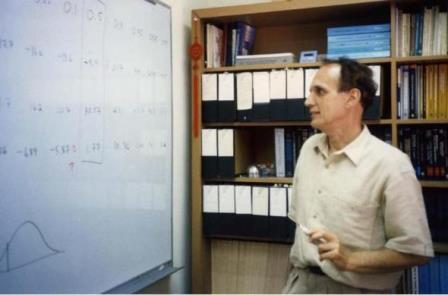
\includegraphics[scale=1]{images/1996_Efron-office}\\
{\tiny Bradley Efron working in his classic office, circa 1996.}

\end{frame}
%===========================================================
\begin{frame}[fragile]\frametitle{References}

\bi
\item \href{https://statprize.org/}{International Prize in Statistics 2019}
\item \href{https://www.fox.temple.edu/wp-content/uploads/2021/07/Efron-2020-JASA-wdiscussion.pdf}{Efron, B. (2020). Prediction, Estimation, and Attribution. Journal of the American Statistical Association, 115(530), 636-655.} With Discussion and Rejoinder.
\item \href{https://efron.ckirby.su.domains/talks/2019Predict-Estimat-Attribut.pdf}{Slides}
\item \href{https://drive.google.com/file/d/1uknyN7L8rIPCcyxGoXkMlVRE8lh5RFrm/view}{Recorded presentation} for the 62nd ISI World Statistics Congress in Kuala Lumpur [46 mins]
\ei

\end{frame}
%===========================================================
\begin{frame}[fragile]\frametitle{Outline}

\be
\item Introduction
\item Surface Plus Noise Models
\item The Pure Prediction Algorithms
\item A Microarray Prediction Problem
\item Advantages and Disadvantages of Prediction
\item The Training/Test Set Paradigm
\item Smoothness
\item A Comparison Checklist
\item TraditionalMethods in the Wide Data Era
\item Two Hopeful Trends
\ee

\end{frame}
%===========================================================
\begin{frame}[fragile]\frametitle{Regression\\
Gauss (1809), Galton (1877)}

What are the three important statistical tasks in regression?

\end{frame}
%===========================================================
\begin{frame}[fragile]
\begin{itemize}
\item \emph{Prediction: the prediction of new cases}

e.g. random forests, boosting, support vector machines,
neural nets, deep learning

\item \emph{Estimation: the
estimation of regression surfaces}

e.g. OLS, logistic regression, GLM: MLE

\item \emph{Attribution: the assignment of significance
to individual predictors}

e.g. ANOVA, lasso, Neyman Pearson
\end{itemize}

\end{frame}
%===========================================================
\begin{frame}[fragile]

How do the pure prediction algorithms relate to traditional
regression methods?

That is the central question pursued in
what follows.

\end{frame}
%===========================================================
\begin{frame}[fragile]

\bi
\item[2.] Surface Plus Noise Models
\ei

\end{frame}
%===========================================================
\begin{frame}[fragile]

We will assume that the data $\mathbf{d}$ available to the statistician
has this structure:
$$\mathbf{d} = \{(x_i,y_i), i=1,\ldots,n\}$$
\bi
\item  $x_i$ is a $p$-dimensional vector of predictors taking its value
in a known space $\mathcal{X}$ contained in $\mathbb{R}^p$;
\item $y_i$ is a real valued response;
\item the $n$ pairs are assumed to be independent of each
other.
\ei
More concisely we can write
$$\mathbf{d} = \{\mathbf{x},\mathbf{y}\}$$
where $\mathbf{x}$ is the $n\times p$ matrix having $x_i^t$ as the $i$th row, and $\mathbf{y}=(y_1,\ldots,y_n)^t$.


\end{frame}
%===========================================================
\begin{frame}[fragile]

\bi
\item The regression model is
\begin{eqnarray}
y_i = s(x_i,\beta) + \epsilon_i \quad i=1,\ldots,n
\end{eqnarray}
$\epsilon_i \stackrel{\mathrm{iid}}{\sim}\mathcal{N}(0,\sigma^2)$
where $s(x,\beta)$ is some functional form that, for any fixed
value of the parameter vector $\beta$, gives expectation $\mu=s(x,\beta)$ as a function of $x\in \mathcal{X}$; 

\item The \emph{regression surface} is
$$\mathcal{S}_\beta = \{\mu=s(x,\beta), x\in \mathcal{X}\}$$
Most traditional regression methods depend on some sort of
surface plus noise formulation;

\item The surface describes the scientific truths
we wish to learn, but we can only observe points on the surface
obscured by noise;

\item The statistician’s traditional estimation task is to learn as much as possible about the surface from the
data $\mathbf{d}$.
\ei

\end{frame}
%===========================================================
\begin{frame}[fragile]

The left panel of the Figure shows the surface representation of
a scientific icon, Newton’s second law of motion,

acceleration = force / mass

It is pleasing to imagine the second law falling full-born out of
Newton’s head, but he was a master of experimentation. The
right panel shows a (fanciful) picture of what experimental data
might have looked like.

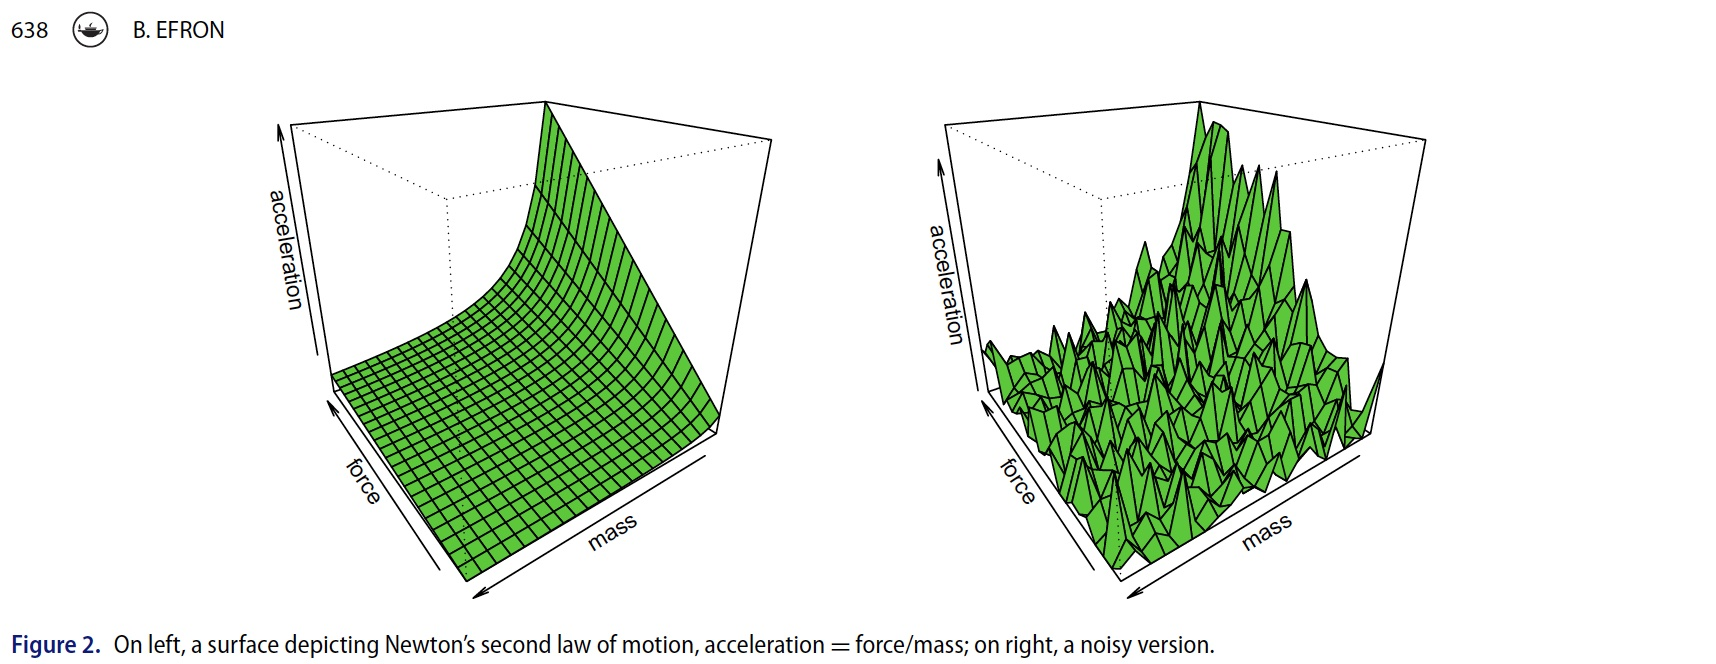
\includegraphics[scale=.2]{images/Figure_2}

\end{frame}
%===========================================================
\begin{frame}[fragile]\frametitle{Cholesterol data}

\bi
\item Cholestyramine, a proposed cholesterol lowering drug, was administered to 164 men for an average of seven years each.

\item The response variable is a man's decrease in cholesterol level over the course of the experiment.

\item The single predictor is compliance, the fraction of intended dose actually taken (standardized)

\item https://hastie.su.domains/CASI\_files/DATA/cholesterol.html
\ei

\end{frame}
%===========================================================
\begin{frame}[fragile]

\centering
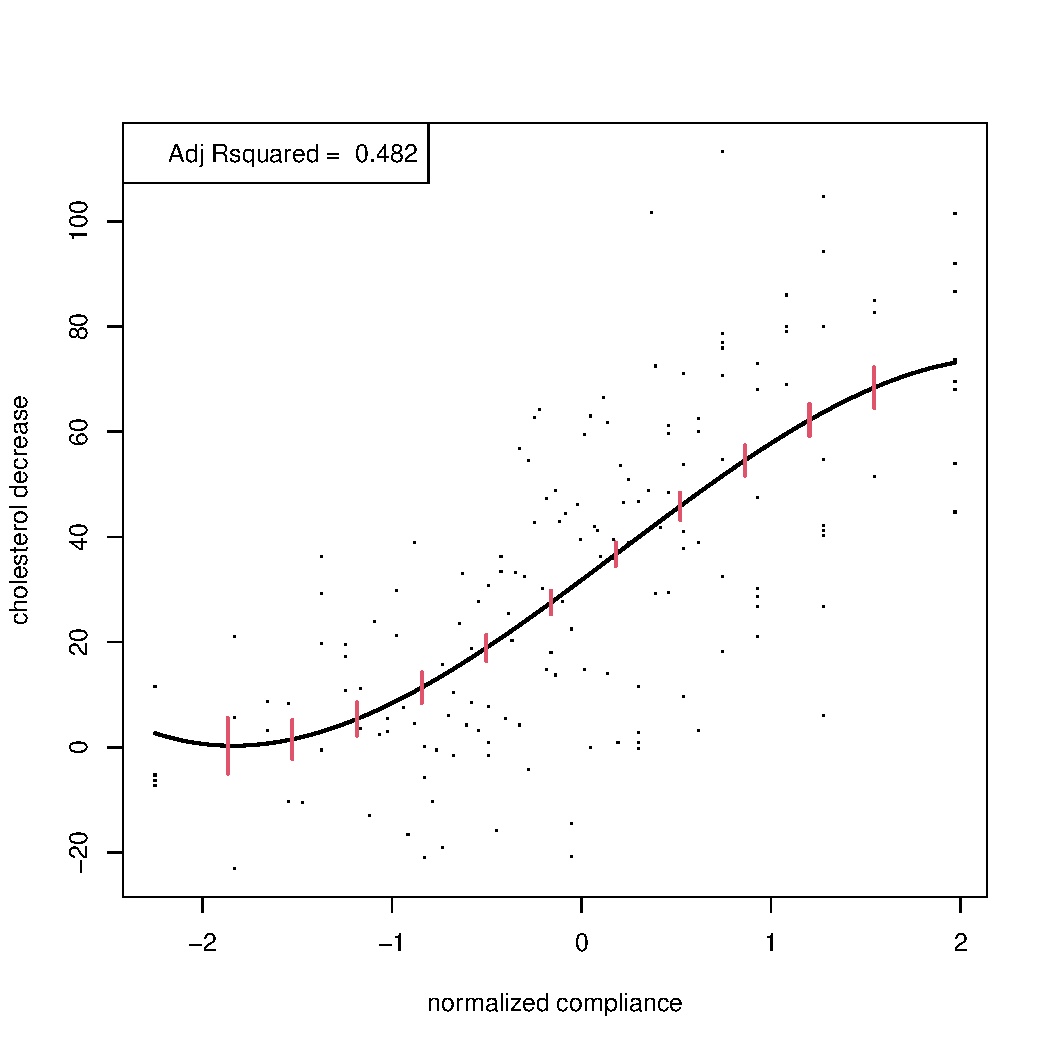
\includegraphics[scale=.45]{images/Figure_1}

https://github.com/aldosolari/SL/blob/master/docs/RCODE/EfronPEA.R

\end{frame}
%===========================================================
\begin{frame}[fragile]

\bi
\item The figure shows a small example, taken from a larger dataset in
Efron and Feldman (1991): $n = 164$ male doctors volunteered to
take the cholesterol-lowering drug cholostyramine. 
\item Two numbers
were recorded for each doctor,
$x_i$ = normalized compliance and
$y_i$ = observed cholesterol decrease. 
\item Compliance, the proportion of the intended dose actually taken,
ranged from 0\% to 100\%, –2.25 to 1.97 on the normalized scale,
and of course it was hoped to see larger cholesterol decreases for
the better compliers.
\ei

\end{frame}
%===========================================================
\begin{frame}[fragile]

\bi
\item A normal regression model was fit, with
$$s(x_i,\beta)=\beta_0 + \beta_1 x_i + \beta_2 x_i^2 + \beta_3 x_i^3$$ in other words, a cubic regression model.
\item  The black curve is the
estimated surface
$$\hat{\mathcal{S}} = \{s(x,\hat{\beta}), x\in\mathcal{X}\}$$
fit by maximum likelihood or, equivalently, by ordinary least
squares (OLS). 
\item The vertical bars indicate one standard error
for the estimated values $s(x,\hat{\beta})$, at 11 choices of $x$, showing how
inaccurate $\hat{\mathcal{S}}$ might be as an estimate of the true $\mathcal{S}$. That is the estimation side of the story. 
\item As far as attribution
is concerned, only $\hat{\beta}_0$ and $\hat{\beta}_1$ were significantly nonzero. The
adjusted $R^2$ was 0.482, a traditional measure of the model’s
predictive power.
\ei

\end{frame}
%===========================================================
\begin{frame}[fragile]\frametitle{\texttt{birthwt} data}

\bi
\item R package \texttt{MASS}
\item The birthwt data frame has 189 rows and 10 columns. 
\item The data were collected at Baystate Medical Center, Springfield, Mass during 1986.
\ei

\end{frame}
%===========================================================
\begin{frame}[fragile]

\bi
\item Another mainstay of traditional methodology is logistic
regression. 
\item The dataset concerns the Risk Factors Associated with Low Infant Birth Weight: $n = 189$ babies, 59 with birth weight less than 2.5 kg and 130 with more than 2.5 kg.
\item Eight covariates were measured at entry: mother's age in years, mother's weight in pounds at last menstrual period, 
body weight, etc., so $x_i$ was 8-dimensional,
while $y_i$ equaled 0 or 1 
\item This is a surface plus noise model, with a linear logistic surface and Bernoulli
noise.
\ei

\end{frame}
%===========================================================
\begin{frame}[fragile]

\begin{table}[ht]
\centering
\begin{tabular}{rlrrrr}
  \hline
 & term & estimate & std.error & p.value & \\ 
  \hline
1 & (Intercept) & 1.07 & 1.27 & 0.40 \\ 
  2 & age & -0.04 & 0.04 & 0.31 \\ 
  3 & lwt & -0.02 & 0.01 & 0.02 & *\\ 
  4 & raceblack & 1.12 & 0.54 & 0.04 & *\\ 
  5 & raceother & 0.67 & 0.47 & 0.16 \\ 
  6 & smoke & 0.75 & 0.43 & 0.08 \\ 
  7 & ptl & -1.66 & 0.90 & 0.07 \\ 
  8 & ht & 1.93 & 0.73 & 0.01 & **\\ 
  9 & ui & 0.80 & 0.48 & 0.09 \\ 
  10 & ftv1 & -0.52 & 0.49 & 0.29 \\ 
  11 & ftv2+ & 0.10 & 0.46 & 0.83 \\ 
  12 & ptd & 3.41 & 1.22 & 0.01 & **\\ 
   \hline
\end{tabular}
\end{table}

\end{frame}
%===========================================================
\begin{frame}[fragile]

\be
\item[3.] The Pure Prediction Algorithms
\ee

\end{frame}
%===========================================================
\begin{frame}[fragile]

\bi
\item Random Forests, Boosting, Deep Learning, etc.

\item Data $$\mathbf{d} = \{(x_i,y_i), i=1,\ldots,n\}$$

\item Prediction rule $f(x,\mathbf{d})$

\item New $(x,?)$ gives $\hat{y} = f(x,\mathbf{d})$

\item Strategy: Go directly for high predictive accuracy;
forget (mostly) about surface + noise

\ei

\end{frame}
%===========================================================
\begin{frame}[fragile]\frametitle{CART}

\centering
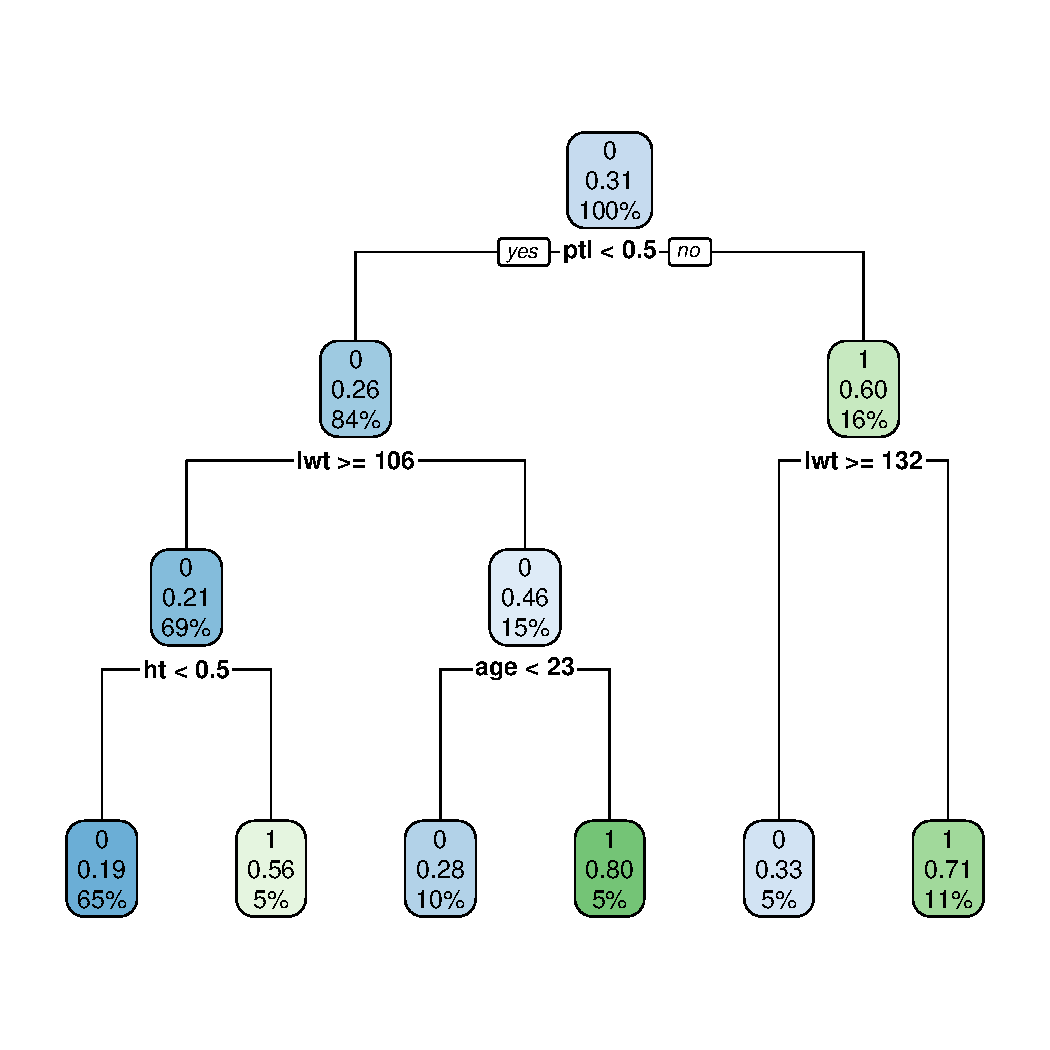
\includegraphics[scale=.45]{images/Figure_3}

\end{frame}
%===========================================================
\begin{frame}[fragile]\frametitle{Random forest}

\centering
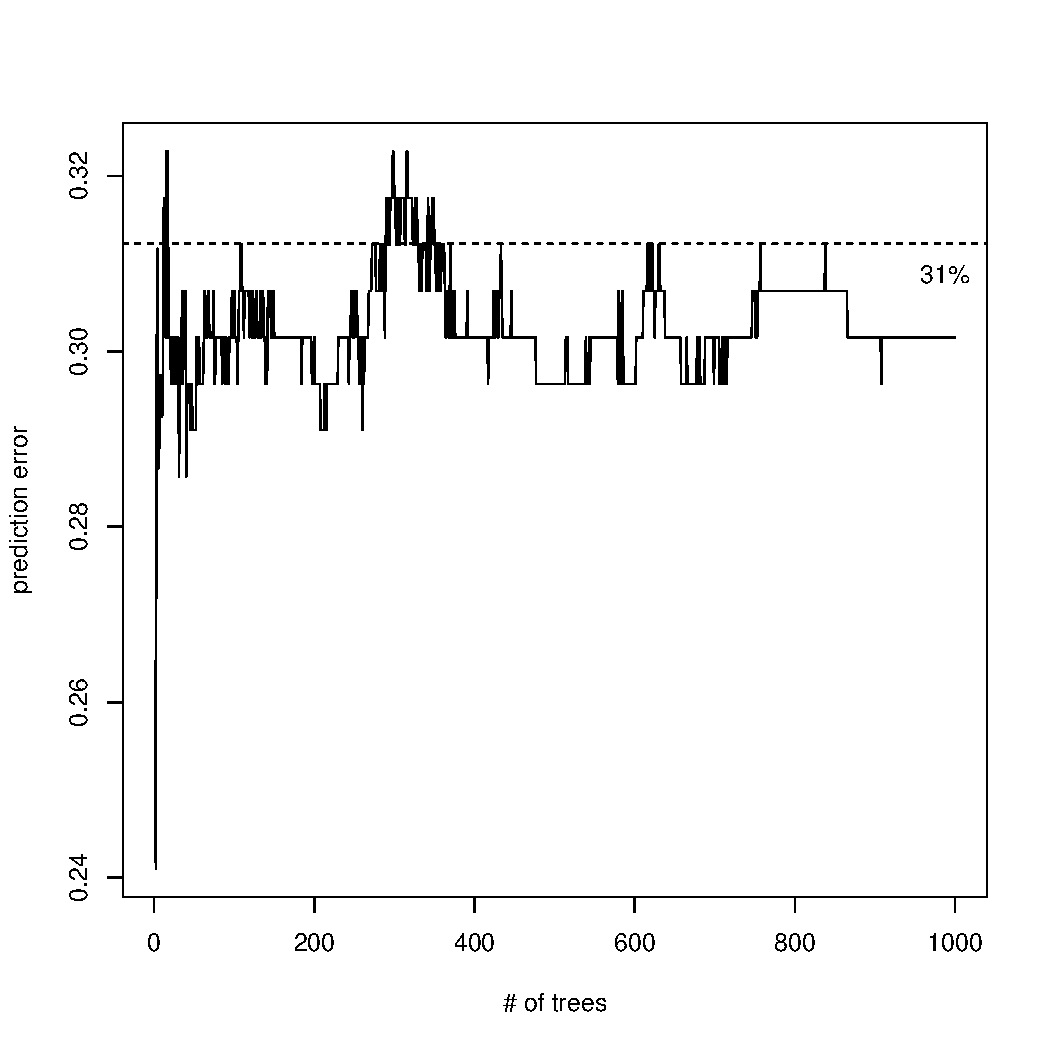
\includegraphics[scale=.45]{images/Figure_4}

\end{frame}
%===========================================================
\begin{frame}[fragile]\frametitle{}

\centering
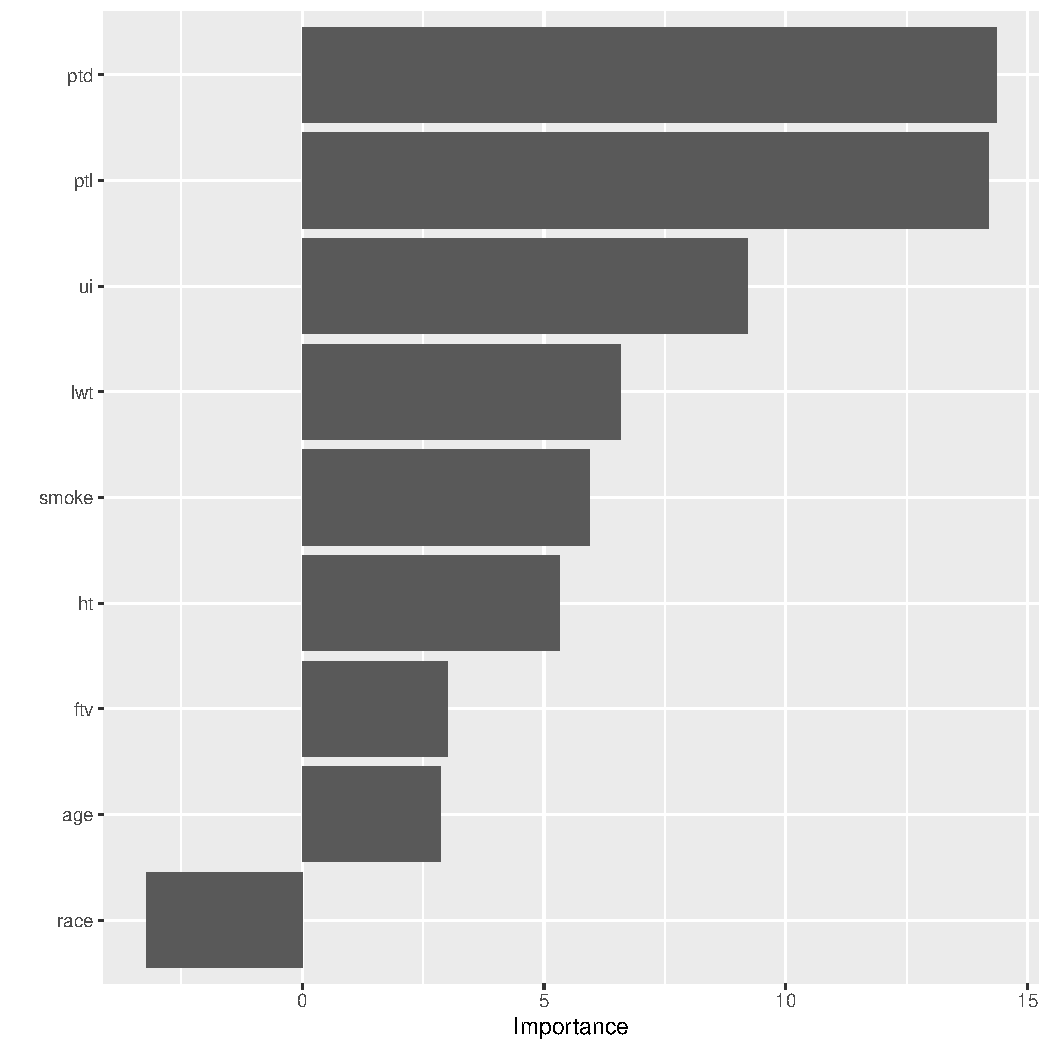
\includegraphics[scale=.45]{images/rf_vip}

\end{frame}
%===========================================================
\begin{frame}[fragile]

Apparent error rate (training error)
$$\widehat{\textrm{err}} = \#\{ f(x_i, \mathbf{d}) \neq y_i\} / n$$

\begin{tabular}{rllr}
  \hline
 & model &  error rate \\ 
  \hline
1 & rand\_forest &0.222  \\ 
  2 & logistic\_reg & 0.243  \\ 
  3 & decision\_tree  &0.228 \\ 
   \hline
\end{tabular}

True error rate
$$E(f(X, \mathbf{d}) \neq Y)$$
where $(X, Y)$ is a random draw from whatever probability
distribution gave the $(x_i, y_i)$ pairs in $\mathbf{d}$;

Estimated by 10-fold cross-validated error rate

\begin{tabular}{rllrrr}
  \hline
 & model  & mean & n & std\_err \\ 
  \hline
1 & rand\_forest  & 0.312 &  10 & 0.04 \\ 
  2 & logistic\_reg  & 0.313 &  10 & 0.03 \\ 
  3 & decision\_tree  & 0.365 &  10 & 0.04 \\ 
   \hline
\end{tabular}

\end{frame}
%===========================================================
\begin{frame}[fragile]

\be
\item[4.] A Microarray Prediction Problem
\ee

\end{frame}
%===========================================================
\begin{frame}[fragile]\frametitle{The Prostate Cancer Microarray Study}

\bi

\item https://hastie.su.domains/CASI\_files/DATA/prostate.html

\item $n = 100$ men: 50 prostate cancer, 50 normal controls

\item For each man measure activity of $p = 6033$ genes

\item Data set $\mathbf{d}$ is $100\times6033$ matrix (``wide'')

\item Wanted: Prediction rule $f(x, \mathbf{d}) $ that inputs new 6033-vector x
and outputs $\hat{y}$ correctly predicting cancer/normal

\ei

\end{frame}
%===========================================================
\begin{frame}[fragile]\frametitle{Random forest}

\bi

\item Randomly divide the 102 subjects into:

\bi
\item  training set of 51 subjects (25 + 25)
\item  test set of 51 subjects (25 + 25)
\ei

\item Run R program \texttt{randomForest} on the training set

\item Use its rule $f(x_i, \mathbf{d})$ on the test set and see how many
errors it makes

\ei

\end{frame}
%===========================================================
\begin{frame}[fragile]

\centering
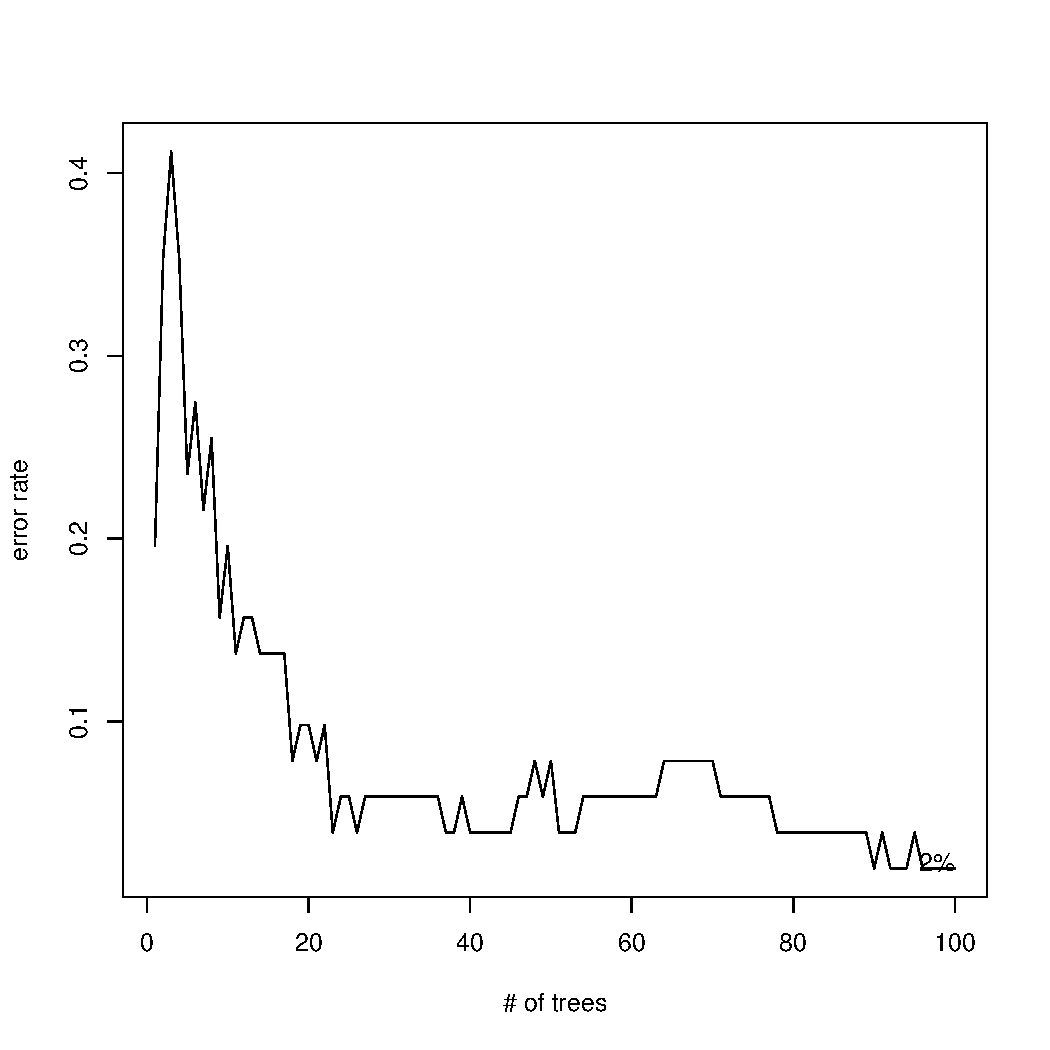
\includegraphics[scale=.45]{images/Figure_5}

\end{frame}
%===========================================================
\begin{frame}[fragile]\frametitle{Boosting}

\centering
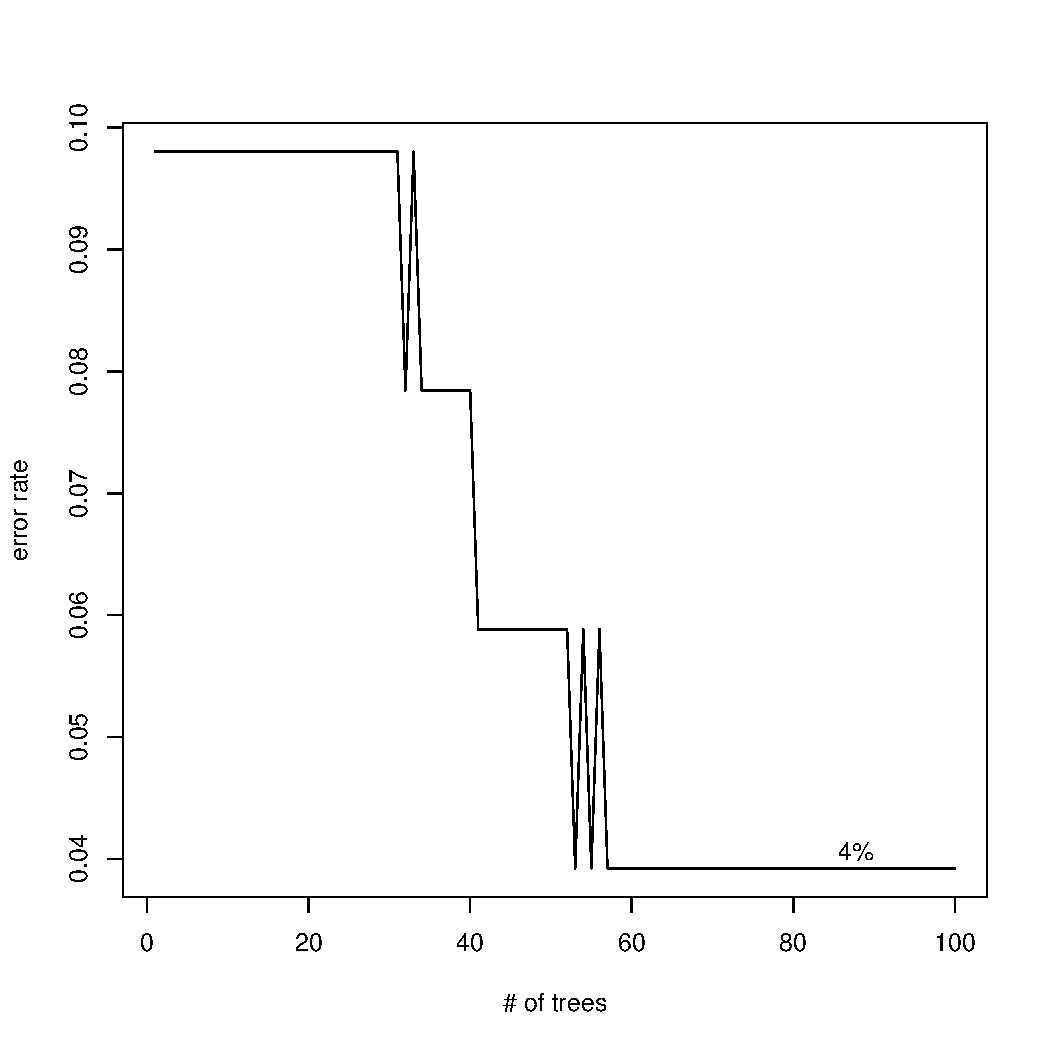
\includegraphics[scale=.45]{images/Figure_6}

\end{frame}
%===========================================================
\begin{frame}[fragile]

\be
\item[5.] Advantages and Disadvantages of Prediction
\ee

\end{frame}
%===========================================================
\begin{frame}[fragile]

\centering
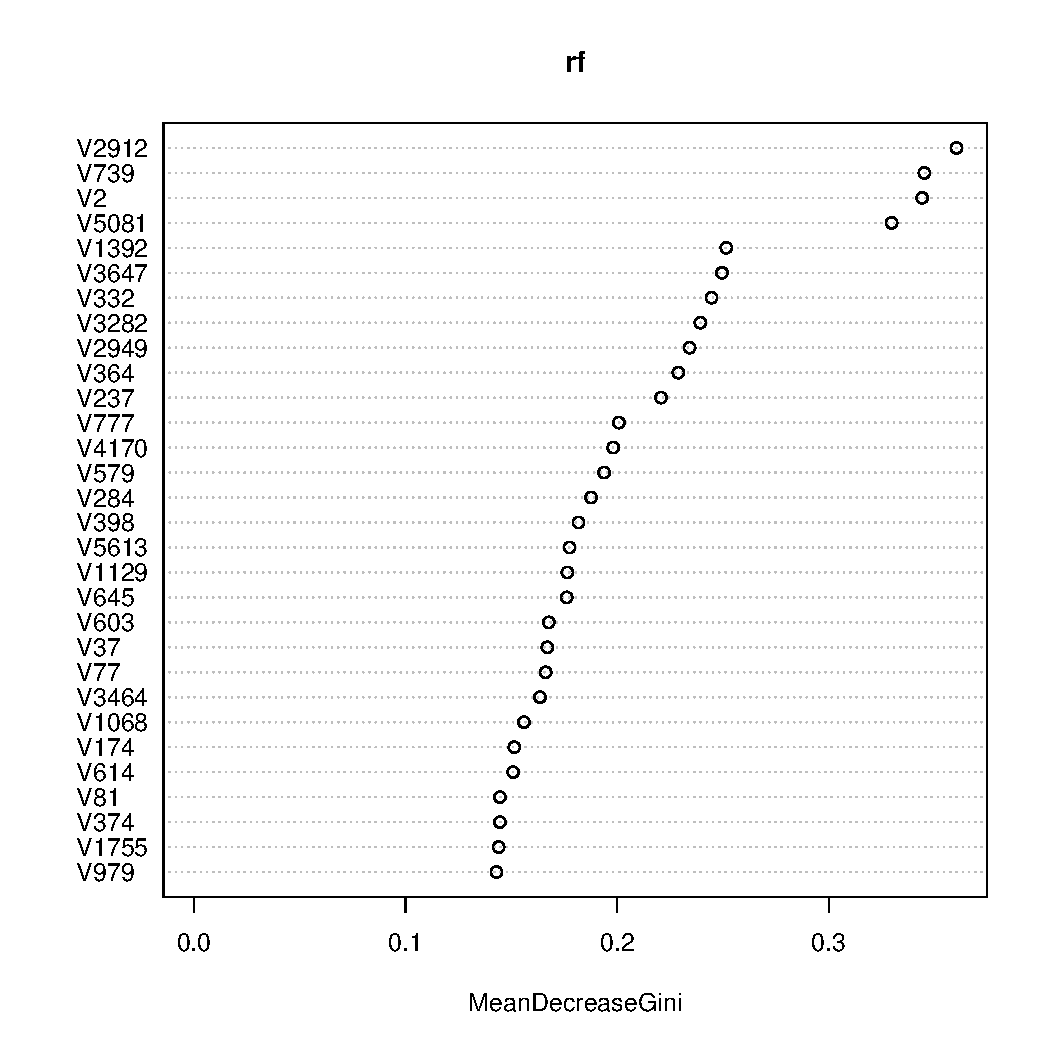
\includegraphics[scale=.45]{images/rf_vip_prostate}

\end{frame}
%===========================================================
\end{document}










